\documentclass[
	% -- opções da classe memoir --
	article,			% indica que é um artigo acadêmico
	12pt,				% tamanho da fonte
	oneside,			% para impressão apenas no verso. Oposto a twoside
	a4paper,			% tamanho do papel. 
	% -- opções da classe abntex2 --
	%chapter=TITLE,		% títulos de capítulos convertidos em letras maiúsculas
	section=TITLE,		% títulos de seções convertidos em letras maiúsculas
	subsection=TITLE,	% títulos de subseções convertidos em letras maiúsculas
	%subsubsection=TITLE % títulos de subsubseções convertidos em letras maiúsculas
	% -- opções do pacote babel --
	english,			% idioma adicional para hifenização
	brazil,				% o último idioma é o principal do documento
	sumario=tradicional
	]{abntex2}
\usepackage[T1]{fontenc}
\usepackage[scaled]{helvet}
\renewcommand\familydefault{\sfdefault} 
\usepackage[utf8]{inputenc}
\usepackage{lmodern,latexsym,enumerate}
\usepackage{amsmath,amsthm,amsopn,amstext,amscd,amsfonts,amssymb}
\usepackage{graphicx}
\usepackage{setspace}
\usepackage{float}
\usepackage{microtype} 
\usepackage{array} % for defining a new column type
 \usepackage{bm}
\usepackage{url}
\usepackage{indentfirst}
\usepackage{bbding}
\usepackage{pifont}
\usepackage{wasysym}
\usepackage{here,color}
\usepackage{lipsum} % 

\usepackage[most]{tcolorbox}
\usepackage{titlesec}
\titleformat{\section}
  {\normalfont\fontsize{12}{15}\bfseries}{\thesection}{1em}{}
\titleformat{\subsection}
  {\normalfont \fontsize{11}{15}\bfseries}{\thesection}{1em}{}
\titleformat{\subsubsection}
  {\normalfont\fontsize{10}{15}\bfseries}{\thesection}{1em}{}


\usepackage[brazilian]{backref}
\usepackage[alf,abnt-full-initials=no,abnt-emphasize=bf,abnt-repeated-author-omit=no]{abntex2cite}

% Paginas com as citações na bibl

% Configurações do pacote backref
% Usado sem a opção hyperpageref de backref
%\renewcommand{\backrefpagesname}{Citado na(s) página(s):~}
% Texto padrão antes do número das páginas
%\renewcommand{\backref}{}
% Define os textos da citação
%\renewcommand*{\backrefalt}[4]{
%	\ifcase #1 %
%		Nenhuma citação no texto.%%
%	\or
%		Citado na página #2.%
%	\else
%		Citado #1 vezes nas páginas #2.%
%	\fi}%
% ---

\renewcommand{\bibsection}{\section*{REFERÊNCIAS}}


\usepackage{xcolor}
% Definindo novas cores
\definecolor{verde}{rgb}{0,0.5,0}
% Configurando layout para mostrar codigos C++, R,...
\usepackage{listings}
\lstset{
  language=C++,
  basicstyle=\ttfamily\small,
  keywordstyle=\color{blue},
  stringstyle=\color{verde},
  commentstyle=\color{red},
  extendedchars=true,
  showspaces=false,
  showstringspaces=false,
  numbers=left,
  numberstyle=\tiny,
  breaklines=true,
  backgroundcolor=\color{green!10},
  breakautoindent=true,
  captionpos=b,
  xleftmargin=0pt,
}

%%%%%%%%%%%%%%%%%%%%%%%%%%%%%%%%%%%%%%%%%%%%%%%%
%Configuração da Primeira Pagina 
%%%%%%%%%%%%%%%%%%%%%%%%%%%%%%%%%%%%%%%%%%%%%%%
\makeatletter
\newlength\drop
\newcommand*{\titleIC}{%
\thispagestyle{empty}
\begingroup% Gentle Madness
\drop = 0.1\textheight
\vspace*{-3cm}
\begin{center}
XVII Congresso de Iniciação Científica da Universidade Federal de Campina Grande    
\end{center}
\hbox{

\includegraphics[width=2.25cm,height=2.22cm]{ufcg.png}
\hspace*{0.55\textwidth}

\includegraphics[width=4.cm,height=2.22cm]{cnpq.png}
}
\begin{center}
 \normalfont\fontsize{12}{15}\bfseries\@title\par  
\end{center}
\vspace{5pt}
\begin{flushright}
\normalfont\fontsize{10}{15}\bfseries\@author\par
\end{flushright}
\vspace{5pt}
\thispagestyle{empty}\@thanks
\endgroup
}
\makeatother
%%%%%%%%%%%%%%%%%%%%%%%%%%%%%%%%%%%%%%%%%%%%%%%%%

%%%%%%%%%%%%%%%%%%%%%%%%%%%%%%%%%%%%%%%%%%%%%%%%
%Configuração da Primeira Pagina 
%%%%%%%%%%%%%%%%%%%%%%%%%%%%%%%%%%%%%%%%%%%%%%%
\makeatletter
\newcommand*{\titleICpagII}{%
\thispagestyle{empty}
\begingroup% Gentle Madness
\drop = 0.1\textheight
\begin{center}
 \normalfont\fontsize{12}{15}\bfseries\@title\par  
\end{center}
\vspace{48pt}
}
\makeatother
%%%%%%%%%%%%%%%%%%%%%%%%%%%%%%%%%%%%%%%%%%%%%%%%%





%%%%%%%%%%%%%%%%%%%%%%%%%%%%%%%%%%%%%%%%%%%%%%%%
\titulo{IDENTIFICAÇÃO DE FALHAS MECÂNICAS EM MÁQUINAS GIRANTES ATRAVÉS DA ANÁLISE, EM NUVEM, DE ASSINATURA VIBRACIONAL}
 
%%%%%%%%%%%%%%%%%%%%%%%%%%%%%%%%%%%%%%%%%%%%5
%
\author{
João Victor Rodrigues Ramalho
\thanks{Aluno do curso de Bacharelado em Engenharia Elétrica, Departamento de Engenharia Elétrica, UFCG, Campina Grande, PB, e-mail: joao.ramalho@ee.ufcg.edu.br}, 
Rafael Bezerra Correia Lima
\thanks{Prof. Dr. do Curso de Engenharia Elétrica,Departamento de Engenharia Elétrica, UFCG, Campina Grande, PB, e-mail: rafael.lima@dee.ufcg.edu.br}
}





% alterando o aspecto da cor azul
\definecolor{blue}{RGB}{41,5,195}
% informações do PDF
\makeatletter
\hypersetup{
     	%pagebackref=true,
		pdftitle={\@title}, 
		pdfauthor={\@author},
    	pdfsubject={Modelo de artigo científico com abnTeX2},
	    pdfcreator={LaTeX with abnTeX2},
		pdfkeywords={abnt}{latex}{abntex}{abntex2}{atigo científico}, 
		colorlinks=true,       		% false: boxed links; true: colored links
    	linkcolor=blue,          	% color of internal links
    	citecolor=blue,        		% color of links to bibliography
    	filecolor=magenta,      		% color of file links
		urlcolor=blue,
		bookmarksdepth=4
}
\makeatother

% --- 

% ---
% compila o indice
% ---
%\makeindex
% ---

% ---
% Altera as margens padrões
% ---
\setlrmarginsandblock{3cm}{2cm}{*}
\setulmarginsandblock{3cm}{2cm}{*}
\checkandfixthelayout
% ---

% --- 
% Espaçamentos entre linhas e parágrafos 
% --- 

% O tamanho do parágrafo é dado por:
\setlength{\parindent}{1.25cm}

% Controle do espaçamento entre um parágrafo e outro:
\setlength{\parskip}{0.2cm}  % tente também \onelineskip

% Espaçamento 
%\SingleSpacing (simples)
\OnehalfSpacing %1,5


%---------
%Estilo Rodapé
%----------
%%criar um novo estilo de cabeçalhos e rodapés
\makepagestyle{estiloUFCG}
\makeevenfoot{estiloUFCG}{}{}{\thepage} 
\makeoddfoot{estiloUFCG}{}{}{\thepage}

%------------
%Configuracao abstract
%------------
\renewenvironment{abstract}
 {\small
\begin{flushleft}
  \bfseries \abstractname\vspace{-.5em}\vspace{0pt}
\end{flushleft}
  \list{}{
    \setlength{\leftmargin}{0cm}%
    \setlength{\rightmargin}{0cm}%
  }%
  \item\relax}
 {\endlist}

% ----
% Início do documento
% ----
\begin{document}





% Retira espaço extra obsoleto entre as frases.
\frenchspacing 

% ----------------------------------------------------------
% ELEMENTOS PRÉ-TEXTUAIS
% ----------------------------------------------------------

%---
%
% Se desejar escrever o artigo em duas colunas, descomente a linha abaixo
% e a linha com o texto ``FIM DE ARTIGO EM DUAS COLUNAS''.
% \twocolumn[    		% INICIO DE ARTIGO EM DUAS COLUNAS
%
%---
% página de titulo
%\setlength{\droptitle}{10pt}
%\maketitle
\titleIC

% resumo em português
\begin{resumo}[\small \textbf{RESUMO}]
A identificação de falhas mecânicas através da assinatura vibracional é um dos principais métodos de monitoramento de condições em máquinas girantes. São técnicas pouco invasivas que garantem uma extensão considerável da vida útil dos equipamentos. Todas as máquinas emitem vibrações durante o seu funcionamento e o processo de leitura e interpretação dessas vibrações evita a necessidade de rotinas de manutenção desnecessárias com trocas de equipamentos que ainda possam ser utilizados. A integração desse modelo de manutenção com a estrutura de Internet Industrial das Coisas (\textit{Industrial Internet of Things}), torna o processo mais acessível e economicamente viável por meio de implementações em serviços de nuvem, como por exemplo o Microsoft Azure. Além da aquisição dos sinais de vibração, é proposto o diagnóstico de falhas por meio da análise remota do espectro de frequência.

 \vspace{\onelineskip}
 \noindent
 \textbf{Palavras-chaves}: Manutenção Preditiva, Análise de vibração, Internet das Coisas, Computação em Nuvem.
\end{resumo}

% ]  				% FIM DE ARTIGO EM DUAS COLUNAS
% ---
% resumo em português



\newpage
\titleICpagII


\begin{resumo}[\small \textbf{ABSTRACT}]
 \begin{otherlanguage*}{english}
The identification of mechanical failures through vibrational signature is one of the main methods of monitoring conditions in rotating machines. They are not very invasive techniques that ensure a considerable extension of the useful life of the equipment. All machines emit vibrations during operation and the process of reading and interpreting these vibrations avoids the need for unnecessary maintenance routines with equipment changes that can still be used. The integration of this maintenance model with the Industrial Internet of Things structure makes the process more accessible and economically viable through implementations in cloud services, such as Microsoft Azure. In addition to the acquisition of vibration signals, fault diagnosis is proposed through remote analysis of the frequency spectrum.
   \vspace{\onelineskip}
 
   \noindent 
   \textbf{Keywords}: Predictive Maintenance, Vibration Analysis, Internet of things, Cloud Computing.
 \end{otherlanguage*}
\end{resumo}


% ----------------------------------------------------------
% ELEMENTOS TEXTUAIS
% ----------------------------------------------------------
\newpage
\textual
\pagestyle{estiloUFCG}

\section*{INTRODUÇÃO}

O projeto  teve como objetivo o desenvolvimento de um sistema de identificação de falhas mecânicas em máquinas girantes, por meio da leitura e análise de sinais de vibração em nuvem. 

A análise de vibração é o método mais utilizado para o monitoramento de máquinas, devido a suas vantagens em comparação a outros métodos. É um procedimento não invasivo, sendo possível identificar a  necessidade de manutenção de forma externa e sem interromper o funcionamento do equipamento. A leitura pode ser continua ou intercalada, sendo assim, é possível identificar falhas instantâneas ou após intervalos de leituras, pelo fato de perceber mudanças no padrões de frequência de vibração, por fim, identificando a falha, como  descrito em MOHANTY (2015). 

%%%%%%%%%%%%%%%%%%%%%%%%%%%%%%%%%%%%%%%%%%%%%%%%%%%%%%%%%%%
\section*{MATERIAIS E MÉTODOS} 

Para o desenvolvimento do projeto foram utilizados os Microcontroladores STM32F401RE (Figura \ref{fig:placa }) e o ESP32(Figura \ref{fig:esp}) , juntamente com o sensor de análise de frequência STEVAL BFA001V1B (STMicroeletronics) (Figura \ref{fig:kit}) .
Como conjunto de softwares foram utilizadas as IDE's (Ambiente de Desenvolvimento Integrado): VsCode(Microsoft), STMCubeIde(ST). Para o desenvolvimento na nuvem foram utilizados as plataformas Microsoft Azure para o recebimento e tratamento de dados e o PowerBI para visualização.

\begin{figure}[H]
    \centering
    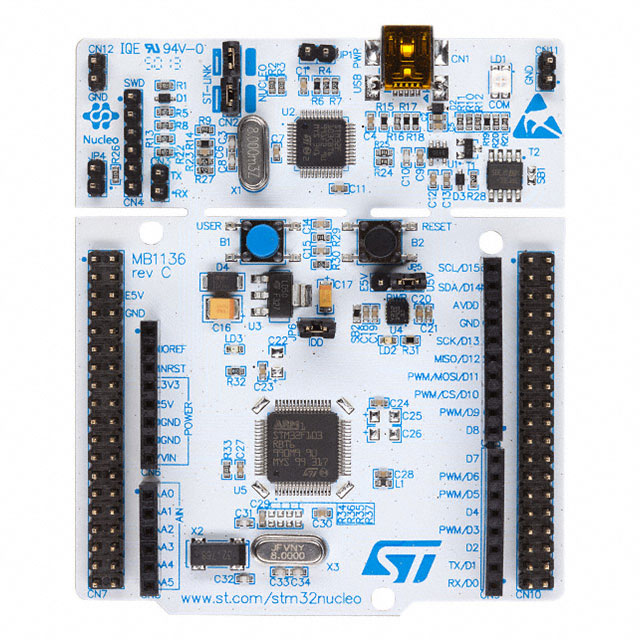
\includegraphics[scale=0.3]{stm32.jpg}
    \caption{Placa STM32 - 401RE}
    \label{fig:placa }
\end{figure}

\begin{figure}[H]
    \centering
    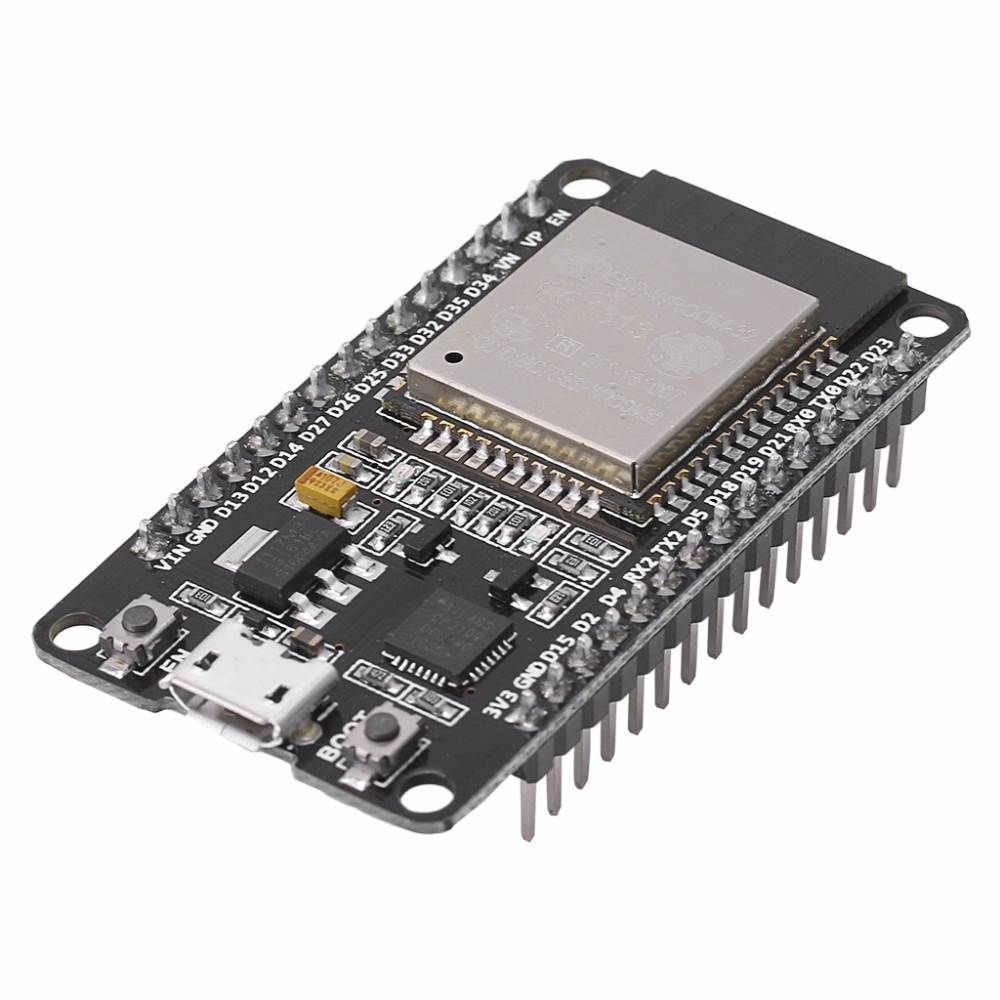
\includegraphics[scale=0.15]{placa_doit_esp32_-_esp-wroom-32_-_wifi_bluetooth.jpg}
    \caption{Placa ESP32}
    \label{fig:esp}
\end{figure}

\begin{figure}[H]
    \centering
    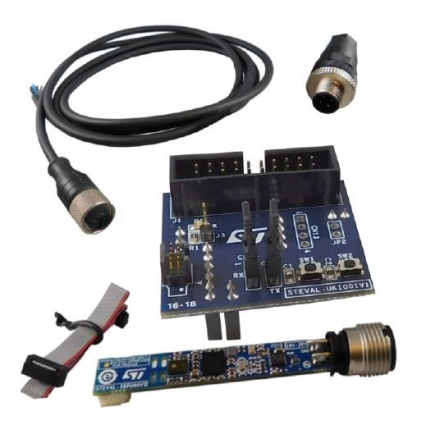
\includegraphics[scale=0.3]{steaval.jpg}
    \caption{Kit STEVAL-BFA001V1B }
    \label{fig:kit}
\end{figure}

\subsection*{STEVAL-BF001V1B}
O sensor STEVAL-BF001V1B é capaz de realizar analise vibracional com a utilização de um acelerômetro digital 3D. O sensor mede a aceleração captada pelo acelerômetro em um intervalo de tempo nas três dimensões, após a leitura é aplicado uma Transformada Rápida de Fourier (FFT), um algoritmo eficiente para realizar o cálculo da Transformada Discreta de Fourier. A FFT consiste em analisar um vetor de amostras no tempo e de acordo com a largura de Banda de Frequência, realizar a transformada para a análise no domínio da frequência, como pode ser exemplificado na Figura \ref{fig:fft}


\begin{figure}[H]
    \centering
    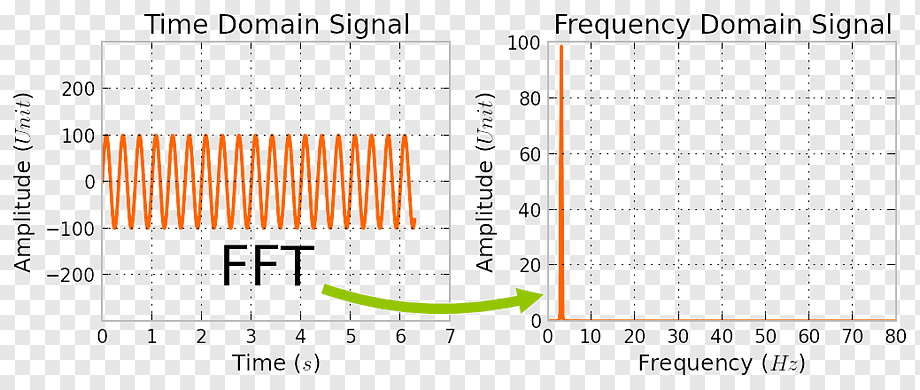
\includegraphics[scale=0.5]{fft.png}
    \caption{Transformada Rápida de Fourier}
    \label{fig:fft}
\end{figure}


%%%%%%%%%%%%%%%%%%%%%%%%%%%%%%%%%%%%%%%%%%%%%%%%%%%%%%%%%%%
\subsection*{Microsoft Azure}
A Microsoft Azure é uma plataforma de multiferramentas de processamento na nuvem, por meio da utilização de processamento e armazenamento em Data Centers. Os serviços utilizados do Microsoft Azure foram: \textit{Azure IoT Hub}, \textit{Azure Stream Analytics Job} e o \textit{Azure Machine Learning Studio}. O principal objetivo em utilizar a Microsoft Azure foi em realizar a integração com da aplicação IoT (\textit{Internet of Things}), com os outros serviços. A internet das coisas, se refere a um modelo de revolução tecnológica em que tende a tornar os dispositivos do dia a dia dos seres humanos mais conectados com a internet, facilitando a comunicação entre humanos e máquinas. Já é possível ver aplicações práticas da rede de internet das coisas atualmente, seja em serviços de assistente de voz, relógios inteligentes, agilização de atendimentos médicos etc. Já para o desenvolvimento com a integração com o Azure Machine Learning Studio.
%%%%%%%%%%%%%%%%%%%%%%%%%%%%%%%%%%%%%%%%%%%%%%%%%
\subsubsection*{Azure Iot Hub}
O Azure Iot Hub é um serviço fornecido pela plataforma Azure que tem como objetivo ser um centro de integração entre dispositivos IoT, fornecendo suporte para a comunicação de dispositivos com a nuvem. A conexão ocorre via wifi, sendo necessária a utilização de uma biblioteca específica para o microcontrolador Esp32 (Microsoft,2020a).
%%%%%%%%%%%%%%%%%%%%%%%%%%%%%%%%%%%%%%%%%%%%%%%%%%
\subsubsection*{Azure Stream Analytics}
O Azure Stream Analytics é serviço fornecido pela plataforma Azure para processamento de eventos e analises em tempo real. Seu principal objetivo foi servir como um canal de comunicação entre o Azure Iot Hub e o PowerBI, sendo possível fazer transmissão e amostragem dos dados em tempo real (Microsoft,2020b).

\subsection*{Azure Machine Learning Studio}
O Azure Machine Learning Studio é uma plataforma intuitiva utilizada para desenvolvimento de algoritmos de Machine Learning, sendo necessário se aprimorar nos principais modelos de aprendizado de máquina utilizando como base Theobald (2017) em seu livro \textit{Machine Learning for Absolute Beginners: A Plain English Introduction}, sendo os principai modelos utilizados na plataforma: Regressão Linear, Classificação, Clustering e Detecção de anomalias.
%%%%%%%%%%%%%%%%%%%%%%%%%%%%%%%%%%%%%%%%%%%%%%%%%%%%%%%%%%%
\subsubsection*{Regressão Linear}
O Modelo de Regressão linear (Figura \ref{fig:Regressao}), consiste em utilizar um algoritmo de aprendizado de máquina, com objetivo de linearizar os dados previamente coletados, com objetivo de predizer onde possivelmente como novos dados se comportam, para isso é definido o coeficiente de determinação ($\beta$), variável responsável por relacionar entrada e saída, sendo possível representar o modelo como uma função linear($y_{i}$), sendo o coeficiente de determinação a inclinação da reta, $\alpha$ representa uma constante que representa a interceptação da reta com o eixo vertical e $\varepsilon _{i}$ representa possíveis erros na medição.
\begin{equation}
    { y_{i}=\alpha +\beta \,X_{i}+\varepsilon _{i}}
\end{equation}

%(DETALHAR OS MÉTODOS EM SUBSEÇÕES)
\begin{figure}[H]
    \centering
    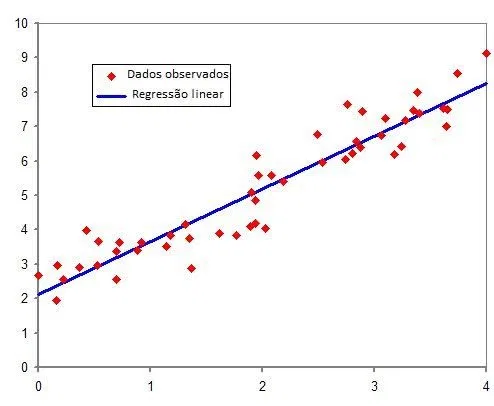
\includegraphics[scale=0.4]{regressao.png}
    \caption{Regressão Linear}
    \label{fig:Regressao}
\end{figure}

%%%%%%%%%%%%%%%%%%%%%%%%%%%%%%%%%%%%%%%%%%%%%%%%%%%%%%%%%%
\subsubsection*{Classificação}
O modelo de Classificação, no qual foi mais abordado o submodelo de Árvore de Decisões (Figura \ref{fig:arvore} ), consiste em o algoritmo traçar uma série de classificações e com isso conseguir organizar os dados em categorias que se agrupam em sub-árvores, como pode ser observado na figura, sendo a última categoria de dados nomeado na posição das folhas da árvore. A maioria dos algoritmos de indução de árvores de decisão trabalha com funções de divisão univariável, ou seja, cada nó interno da árvore é dividido de acordo com um único atributo. Nesse caso, o algoritmo tenta encontrar o melhor atributo para realizar essa divisão

\begin{figure}[H]
    \centering
    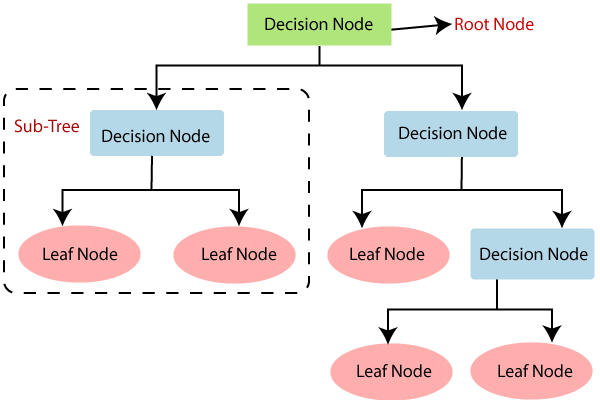
\includegraphics[scale=0.3]{arvore.png}
    \caption{Árvore de Decisões}
    \label{fig:arvore}
\end{figure}
%%%%%%%%%%%%%%%%%%%%%%%%%%%%%%%%%%%%%%%%%%%%%%%%%%%%%%%%%%
\subsubsection*{Clustering}
O modelo de \textit{clustering} (Figura \ref{fig:clus} ), tem como objetivo agrupar dados que possuem categorias semelhantes em grupos, com o objetivo de predizer qual seria o grupo em que um novo dado inserido teria mais possibilidade de participar. Com o objetivo de realizar a organização em forma de grupos, existem diversos métodos de Clustering, dentre eles o \textit{K-means}. O algoritmo \textit{K-means} divide um conjunto de amostras em clusters disjuntos, cada um descrito pela média das amostras no cluster. Os centros dos grupos são normalmente chamados de “centroides” do cluster, sendo assim possível organizar quais elementos se aproximam mais de cada centroide, realizando o agrupamento 

\begin{figure}[H]
    \centering
    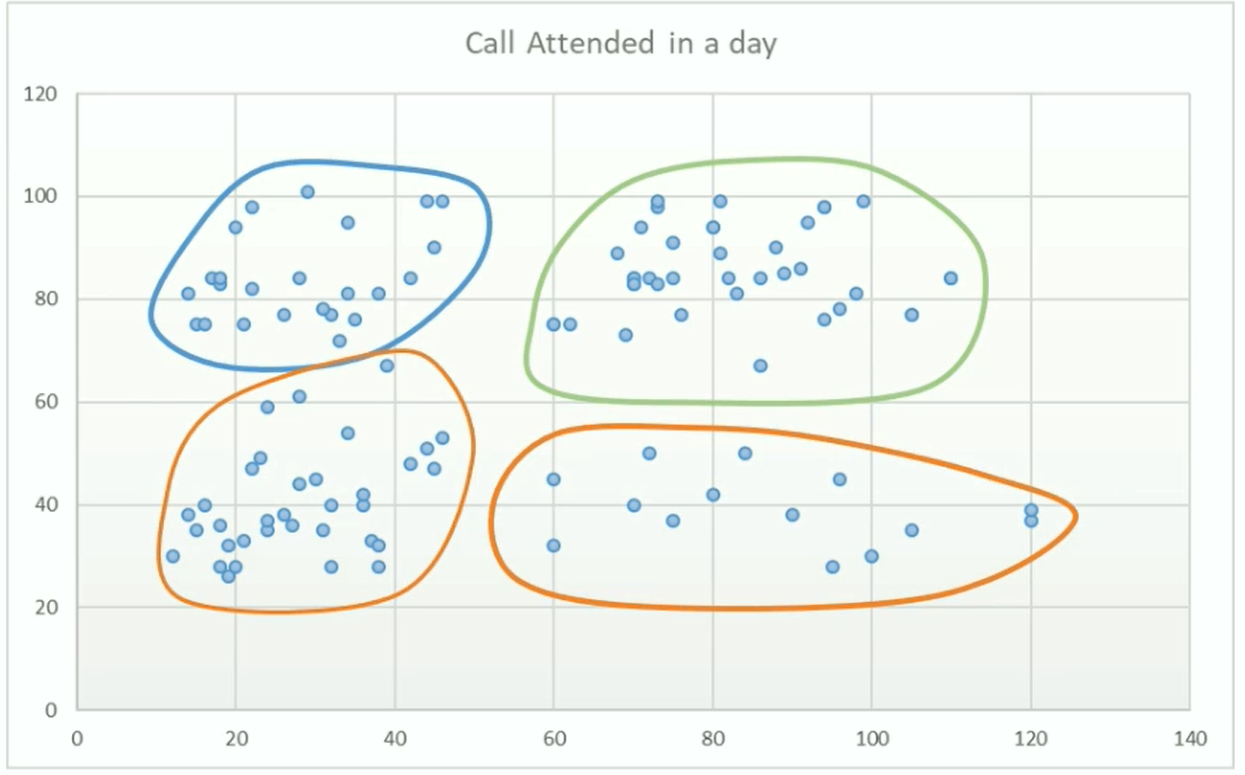
\includegraphics[scale=0.3]{clustering.png}
    \caption{\textit{Clustering}}
    \label{fig:clus}
\end{figure}

%%%%%%%%%%%%%%%%%%%%%%%%%%%%%%%%%%%%%%%%%%%%%%%%%%%%%%%%%
\subsubsection*{Detecção de Anomalias}
Por último o modelo de Detecção de Anomalias (Figura \ref{fig:anomalias} ), tem como objetivo identificar um padrão de fluxo contínuo de dados, buscando apenas identificar anomalias em relação às leituras feitas previamente como pode ser observado na figura \ref{fig:anomalias}. Podendo utilizar dos algoritmos descritos anteriormente, como forma de construir um treinamento rotulado que contém amostras normais e anômalas para construir o modelo preditivo de detecção.

\begin{figure}[H]
    \centering
    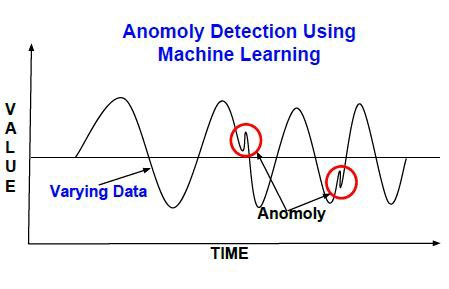
\includegraphics[scale=0.5]{anomaly.png}
    \caption{Detecção de Anomalias}
    \label{fig:anomalias}
\end{figure}
%%%%%%%%%%%%%%%%%%%%%%%%%%%%%%%%%%%%%%%%%%%%%%%%%%%%%%%%%%%%%

\subsection*{Power BI}
O Power BI é uma coleção de serviços de software, que tem como objetivo melhorar a interpretação e visualização de um conjunto de dados, o principal objetivo da utilização da plataforma foi a integração direta com os serviços de IoT fornecidos com pelo Microsoft Azure, tornando a comunicação em tempo real mais eficiente. 

\section*{DESENVOLVIMENTO}
O desenvolvimento do projeto foi realizado em etapas, visto que cada pequeno passo era de extrema importância para todo o projeto,  de início foi realizado um estudo dos códigos base fornecidos  pela plataforma  fabricante do sensor de análise de frequência mostrado na Figura \ref{fig:kit}, a principal mudança necessária nos códigos fornecidos seria  fazer uma limpeza na interface implementada para comunicação com o usuário via prompt de comando (Figura \ref{fig: antes}), para apenas exibição dos dados necessários com  objetivo de implementar o formato de compactação JSON (Figura \ref{fig:json}).


\begin{figure}[H]
    \centering
    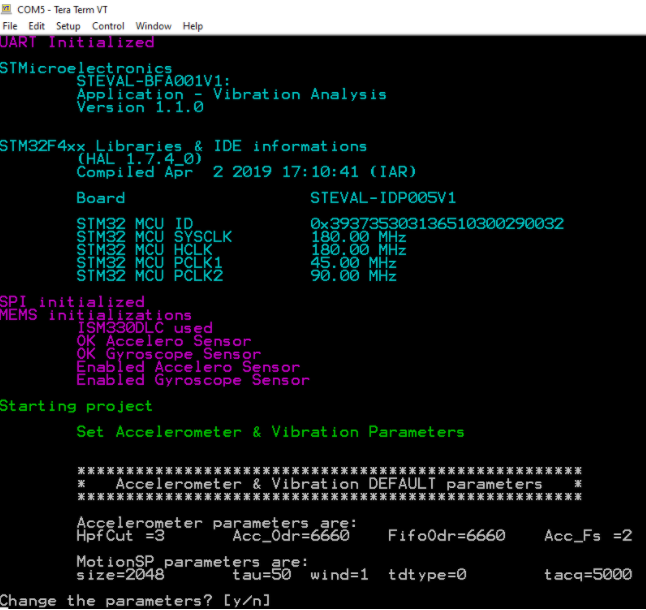
\includegraphics[scale=0.5]{antes.PNG}
    \caption{Código Original}
    \label{fig: antes}
\end{figure}

\begin{figure}[H]
    \centering
    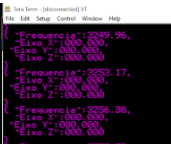
\includegraphics[scale=1.5]{depois.PNG}
    \caption{Formato JSON}
    \label{fig:json}
\end{figure}
A implementação desse formado foi de extrema importância devido à necessidade de comunicação entre os dispositivos, devido a limitações, essa transferência de dados de um microcontrolador para o outro, pois o Esp32 (Figura \ref{fig:esp}) possui conexão com wifi, A comunicação entre os dispositivos foi feita via comunicação serial (Figura \ref{fig:conexao}), o microcontrolador STM32 - F401 RE realizava a leitura juntamente com o kit de sensores de forma compactada enviava esses dados  via serial para o Esp32, que devido a seu módulo de conexão wifi, poderia se conectar diretamente com o Azure IoT Hub, sendo responsável apenas por fazer a ponte entre os Sensores disponíveis no STM com o módulo IoT. 

\begin{figure}[H]
    \centering
    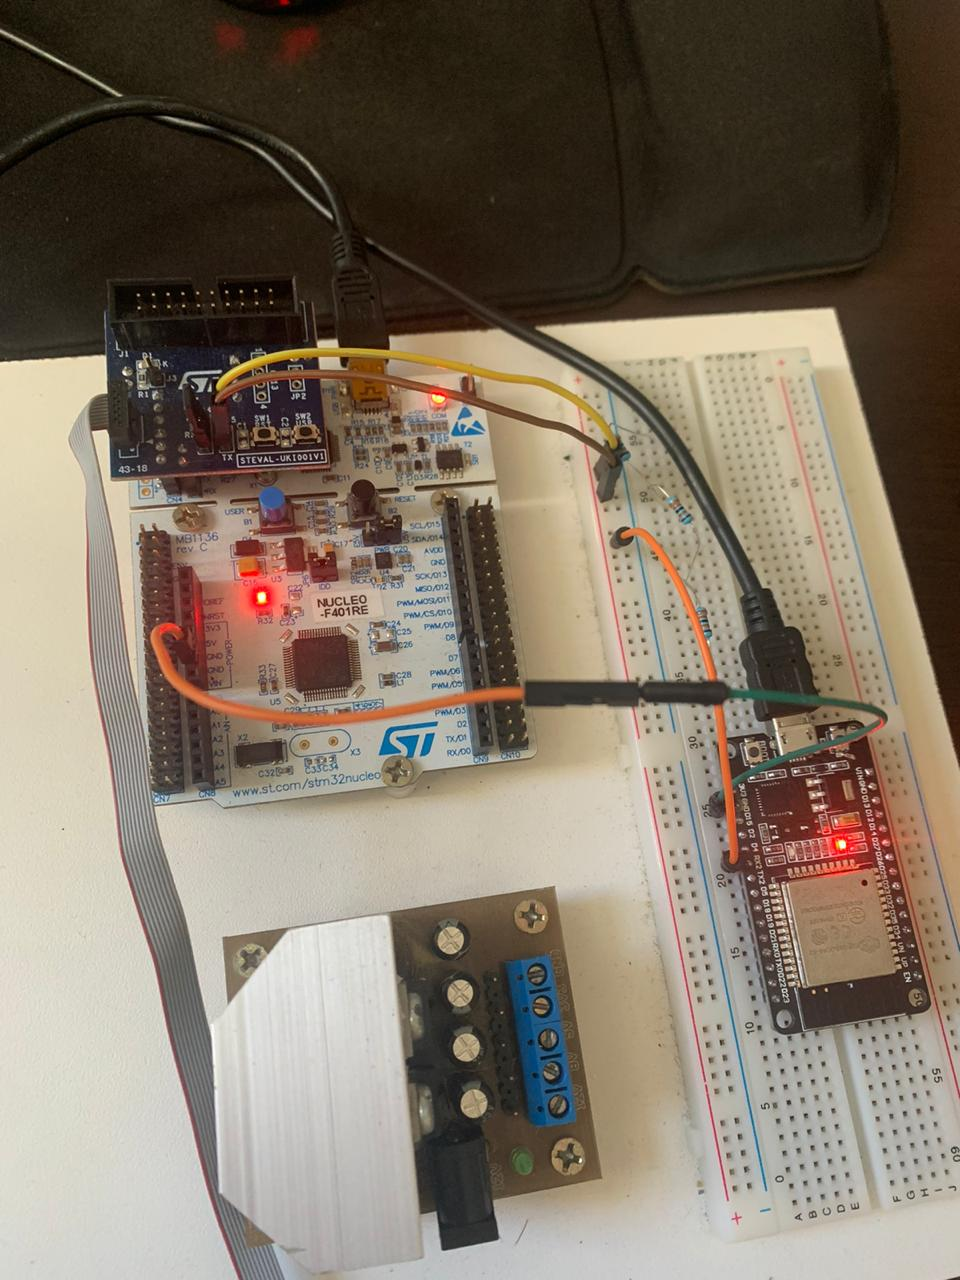
\includegraphics[scale=0.15]{conexao.png}
    \caption{Conexão serial entre o STM e o ESP32}
    \label{fig:conexao}
\end{figure}

Após toda conexão feita, foi necessário fazer o trammit dos dados dentre os pacotes de conexões do azure. O principal deles foi o Stream Analytics, responsável por conectar duas pontas do serviço de Iot, a entrada (Esp32) e a saída(Power BI). O sistema completo pode ser observado na Figura \ref{fig:sistema}

\begin{figure}[H]
    \centering
    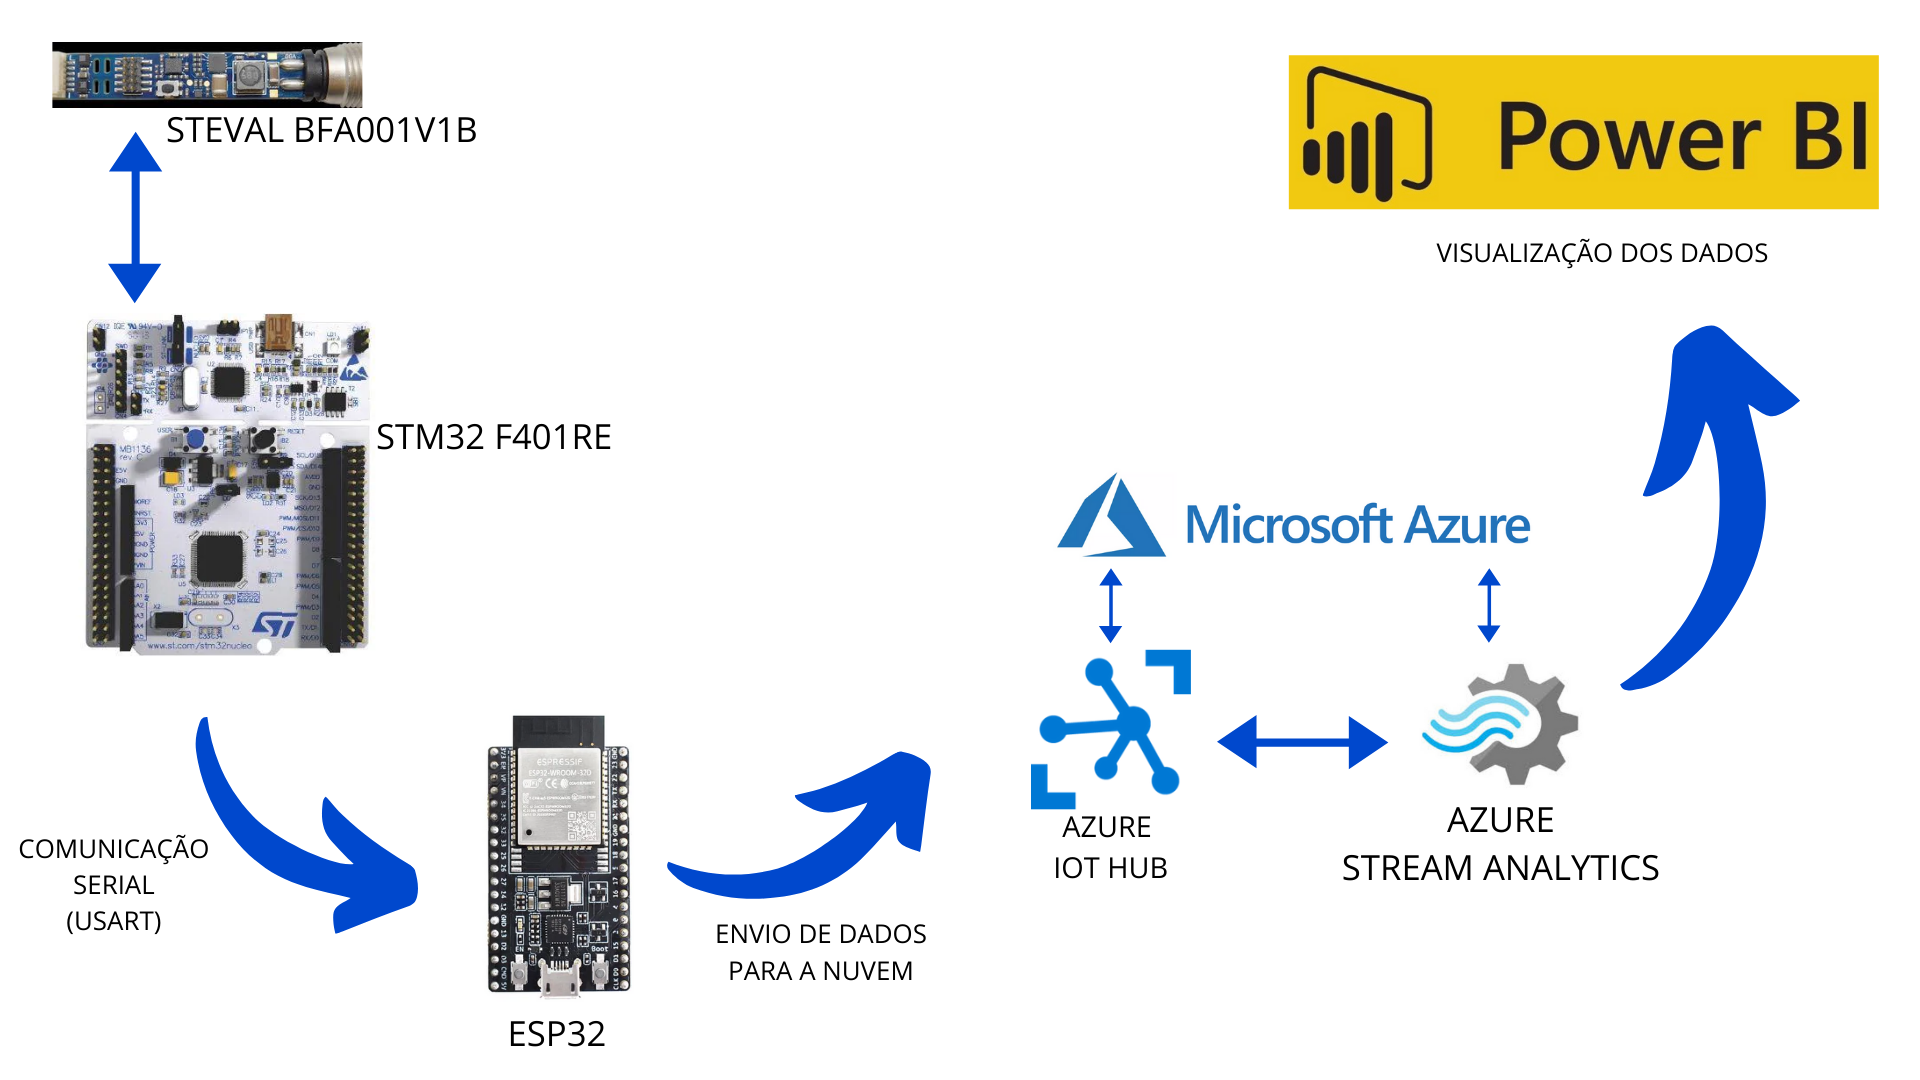
\includegraphics[scale=0.3]{sistema_completo.png}
    \caption{Sistema Completo}
    \label{fig:sistema}
\end{figure}


\section*{RESULTADOS E DISCUSSÕES}
Com todo os procedimentos de \textit{hardware e software} foi possível finalizar o desenvolvimento de uma plataforma Iot com comunicação entre o Sensor de Análise de Frequência, com amostragem em tempo real. Devido às restrições da pandemia as leituras obtidas foram apenas simuladas, não sendo possível fazer leituras reais na máquina girante que se encontrava no Laboratório de Instrumentação Eletrônica e Controle (LIEC) - UFCG. Sendo assim, mesmo com a aplicação de uma frequência simulada foi obtido o resultado da Figura \ref{fig:power}. 


\begin{figure}[H]
    \centering
    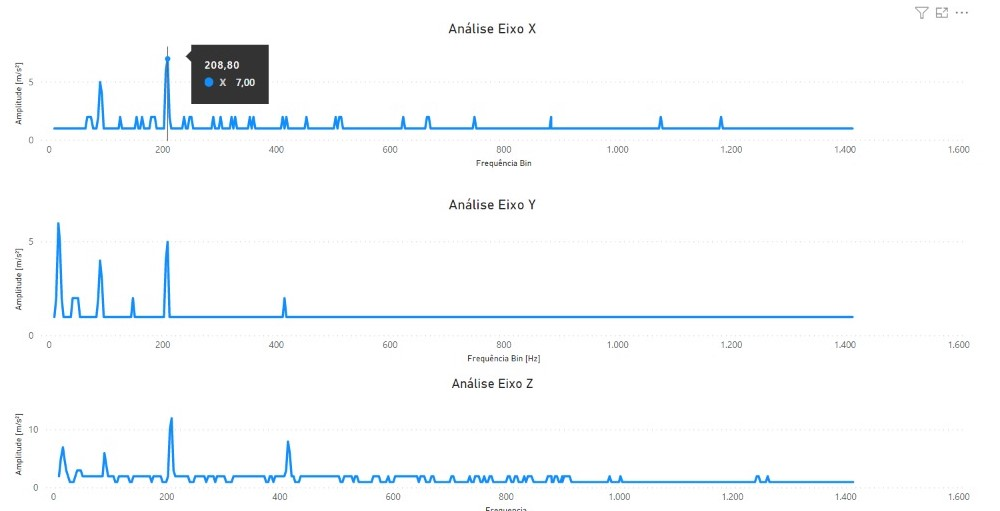
\includegraphics[scale=0.5]{power_bi.jpeg}
    \caption{Dados em tempo real no PowerBI}
    \label{fig:power}
\end{figure}

Para a simulação foi aplicada uma frequência de 200 Hz em uma bancada de madeira, na qual apenas o sensor estava posicionado, o resultado foi que a leitura  foi realizada com sucesso, mostrando os picos de perturbação na frequência aplicada e nas suas harmônicas, de forma semelhante ao que foi mostrado na Figura \ref{fig:fft}. Como continuação do projeto, a implementação dos Algoritmos de Aprendizado de Máquina serão os responsáveis pela a análise preditiva das vibrações, sendo eles responsáveis pela comparação entre leituras e identificação qual tipo de falha mecânica está sendo apresentada, apenas com a análise do gráfico da Amplitude x Frequência. 

\section*{CONCLUSÃO}

O modelo de integração de Internet das Coisas juntamente com a análise vibracional se torna interessante com o objetivo de criar uma rede de sistemas na qual possam ser monitorados de forma integrada, facilitando o processo de identificação de falhas mecânicas. Dessa forma, se torna necessária a continuação desse projeto com objetivo de implementar os processos até aqui desenvolvidos no desenvolvimento de um sistema de monitoramento completo de serviços na nuvem 

\section*{AGRADECIMENTOS}

O presente trabalho foi desenvolvido no programa PIBITI/UFCG 2019/2020 com os agradecimentos ao Dr. Rafael Bezerra Correia Lima pela orientação e dedicação a instituição, aos demais alunos pertencentes ao grupo do Laboratório de Instrumentação Eletrônica e Controle pelo auxílio no desenvolvimento desse projeto.

%\printbibliography[title={Whole bibliography}]
\bibliographystyle{abntex2-alf}
\bibliography{ref}

%(TODAS AS REFERÊNCIAS DEVEM ESTAR CITADAS EM ALGUM PONTO DO TEXTO!!!)


\item[(1)]MOHANTY, A. \textbf{Machinery Condition Monitoring}. Boca Raton, Fla: CRC Press, 2015.

\item [(2)] Theobald, O. \textbf{Machine Learning for Absolute Beginners: A Plain English Introduction}. 2ª. ed. Scatterplot Press, 2017.

\item[(3)]\textbf{Documentação do Servidor de Relatórios do Power BI- Microsoft}. Disponível em: $<$https://docs.microsoft.com/pt-br/power-bi/report-server/$>$. Acesso em:  maio. 2020.

\item[(4)]\textbf{O que é o Azure Stream Analytics?- Microsoft}. Disponível em: $<$https://docs.microsoft.com/pt-br/azure/stream-analytics/stream-analytics-introduction$>$. Acesso em:  maio. 2020.

\item[(5)]\textbf{O que é o Hub IoT do Azure?- Microsoft}. Disponível em: $<$https://docs.microsoft.com/pt-br/azure/iot-hub/about-iot-hub$>$. Acesso em:  maio. 2020.

\item [(6)] Thakur , M. R. \textbf{NodeMCU ESP8266 Communication Methods and Protocols : Programming with Arduino IDE}. Ebook Kindle.



\end{document}
